This layer is responsible for reading the MIDI signals and converting it into audio signals that is needed for the speakers to produce audio output. It consists of MIDI decoder, fluid synth and sound card which are integrated in a Raspberry Pi.

\subsection{Layer Hardware}
It consists of 1.5GHZ quad-core 64-bit raspberry pi.

\subsection{Layer Operating System}
It runs raspbian OS with kernel version 4.19.

\subsection{MIDI Decoder}
It is a driver program that acts as an bridge program between MIDI encoder and the fluidsynth.

\begin{figure}[h!]
	\centering
 	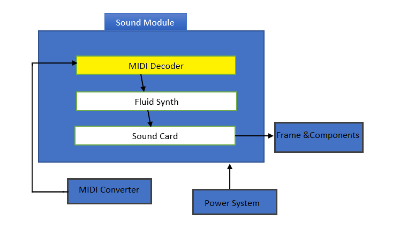
\includegraphics[width=0.60\textwidth]{images/decoder.png}
 \caption{MIDI decoder subsystem description diagram}
\end{figure}

\subsubsection{Subsystem Hardware}
It is running on Raspberry pi 4.

\subsubsection{Subsystem Operating System}
Raspbian OS is running a python 3.6 script that reads the encoding.

\subsubsection{Subsystem Programming Languages}
It uses Python 3.6.0 for server processing which uses socket library for communication with fluidsynth. 

\subsection{Fluidsynth}
Fluidsynth is a real-time MIDI synthesizer based on the SoundFont 2 specifications. 

\begin{figure}[h!]
	\centering
 	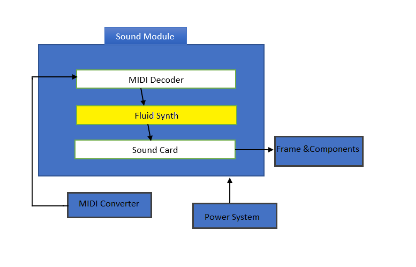
\includegraphics[width=0.60\textwidth]{images/fluidsynth.png}
 \caption{Fluidsynth subsystem description diagram}
\end{figure}

\subsubsection{Subsystem Operating System}
It is runs on startup on a raspbian OS.

\subsubsection{Subsystem Software Dependencies}
Fluidsynth is a library itself which reads in the MIDI input and plays according to the sound font files present. Moreover, socket library is called upon to connect with the fluidsynth process which in turn uses AF\_INET IPV4 protocol for communication.

\subsubsection{Subsystem Programming Languages}
Python is used to call upon the fluidsynth functions to control the gain, reverb and chorus of the audio output. 

\subsection{Soundcard}
Raspberry pi already comes in with a sound card integrated in its system. It is used for converting the output data from fluidsynth to audio data used by speakers for final output.

\begin{figure}[h!]
	\centering
 	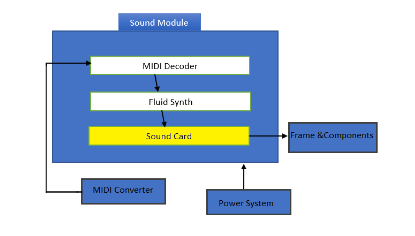
\includegraphics[width=0.60\textwidth]{images/sound card.png}
 \caption{Sound Card subsystem description diagram}
\end{figure}

\subsubsection{Subsystem Hardware}
Raspberry pi 4 with compatible sound drivers for necessary sound processing.

\subsubsection{Subsystem Operating System}
Raspbian OS 








